\section{Nachhaltigkeit}
(noch nicht fertig Timo)

Trotz der Herausforderungen in der Umsetzung konnte ein grosser Teil der in PREN1  definierten Nachhaltigkeitsziele (referenzieren) erfüllt werden. Das Projekt hat gezeigt, dass auch in technisch anspruchsvollen Studierendenprojekten nachhaltiges Handeln möglich und praktikabel ist.

\subsection{3R-Prinzip: Reduce, Reuse, Recycle}
Die in PREN1 definierten Nachhaltigkeitsprinzipien,insbesondere die 3 R (Reduce, Reuse, Recycle), wurden auch in der praktischen Umsetzung in PREN2 angewendet.  

 In diesem Kapitel wird erläutert wie die drei Rs im Verlauf des Semesters umgesetzt wurden.

\subsubsection{Reduce}

Zur weiteren Reduktion des Ressourcenverbrauchs wurde auf papierlose Zusammenarbeit gesetzt. Die gesamte Kommunikation und Dokumentation erfolgte digital. Eine eigene Overleaf-Instanz für die LaTeX-Dokumentation wurde auf einem bereits laufenden Server betrieben, wodurch zusätzlicher Stromverbrauch vermieden werden konnte. Auch das tägliche PDF-Building der Dokumentation wurde bewusst auf ein Minimum reduziert.

Viele Bauteile wie Sensoren, Steckbrettmaterialien, PLA-Filament oder Endschalter waren bereits im Besitz einzelner Teammitglieder und konnten direkt verwendet werden. Dadurch konnten nicht nur unnötige Bestellungen, sondern auch Verpackungsmaterial, Transportwege und Kosten reduziert werden.


\subsubsection{Reuse}

Im Bereich Reuse wurden zahlreiche Elemente des Prototypings direkt in den finalen Roboter übernommen. Dazu zählen etwa die Räder, der Kameraturm und der Greifer. Auch Elektronikkomponenten wie der Raspberry Pi, Sensoren und die Kamera wurden teilweise aus bereits vorhandenen Beständen eingebracht. Die modulare Bauweise erlaubte es, einzelne Bauteile mehrfach zu verwenden und flexibel anzupassen. Beispielsweise konnte die Grundplatte mehrfach verändert werden, ohne ersetzt werden zu müssen. Auch das Konzept, mehrere kleine statt einer grossen Leiterplatte zu verwenden, wurde aus Nachhaltigkeitsgründen beibehalten.



Die Grundplatte des Prototyps aus PREN1 wurde so konstruiert, dass sie modular erweiterbar ist. Zusätzliche Bohrungen und Nuten konnten während der Entwicklung fortlaufend eingebracht werden, ohne dass eine neue Platte gefertigt werden musste. Die Nachbearbeitung mittels Laserschneidmaschine verlief dabei ohne technische Probleme. Dadurch konnte der Materialeinsatz auf eine einzige Grundplatte beschränkt und die Entstehung von Abfall minimiert werden. Eine Übersicht der verschiedenen Bearbeitungszustände ist in Abbildung \ref{fig: Weiterentwicklung der Grundplatte} dargestellt.

\begin{figure}[H] % oder [htbp]
    \centering
    \begin{subfigure}[b]{0.45\textwidth}
        \centering
        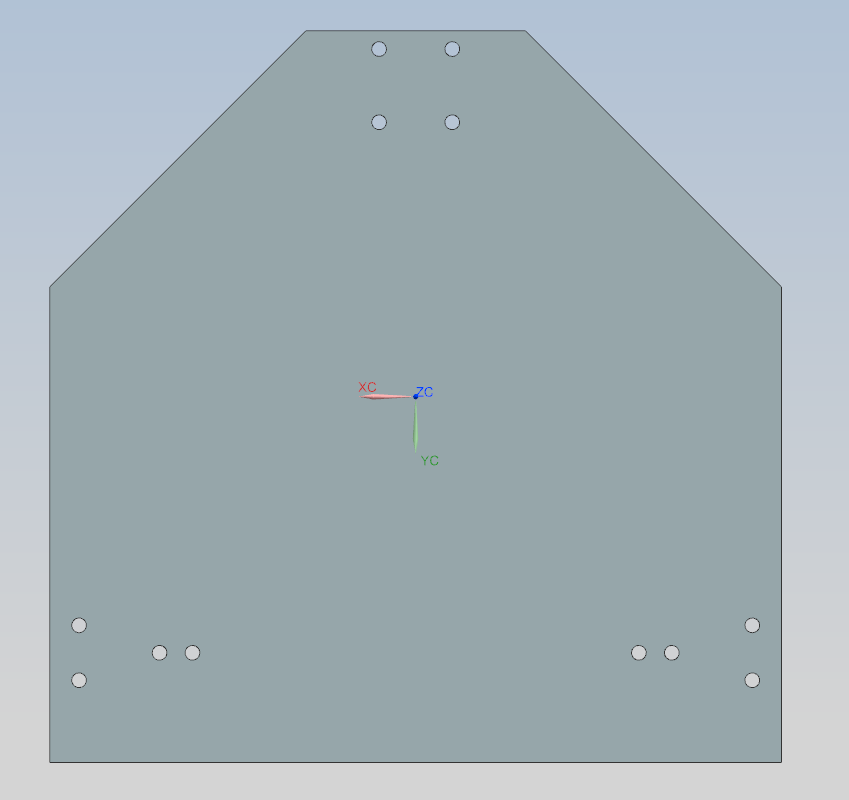
\includegraphics[width=\linewidth]{assets/MT/Grundplatte_V0.png}
        \caption{Grundplatte V0}
    \end{subfigure}
    \hfill
    \begin{subfigure}[b]{0.45\textwidth}
        \centering
        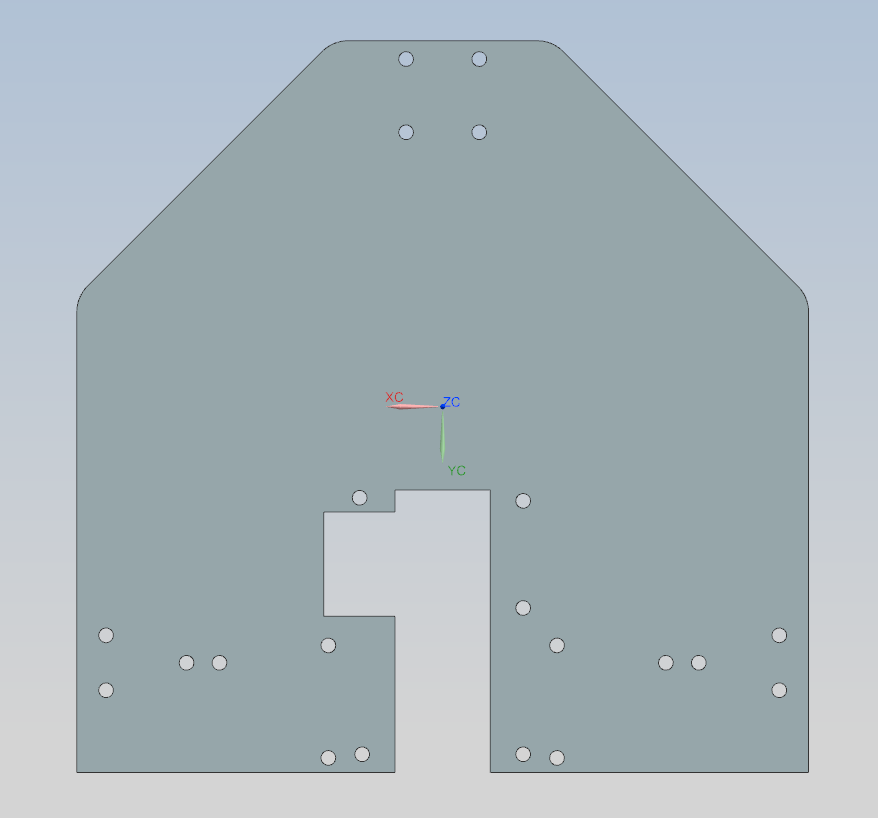
\includegraphics[width=\linewidth]{assets/MT/Grundplatte_V1.png}
        \caption{Grundplatte V1}
    \end{subfigure}

    \vspace{0.5cm}

    \begin{subfigure}[b]{0.45\textwidth}
        \centering
        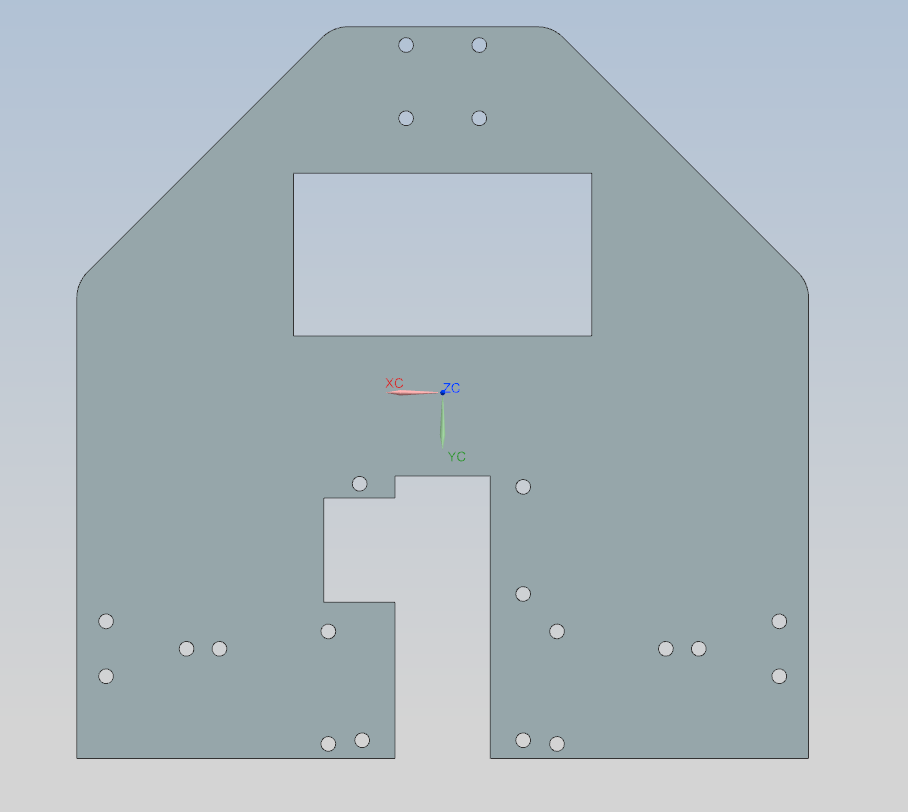
\includegraphics[width=\linewidth]{assets/MT/Grundplatte_V2.png}
        \caption{Grundplatte V2}
    \end{subfigure}
    \hfill
    \begin{subfigure}[b]{0.45\textwidth}
        \centering
        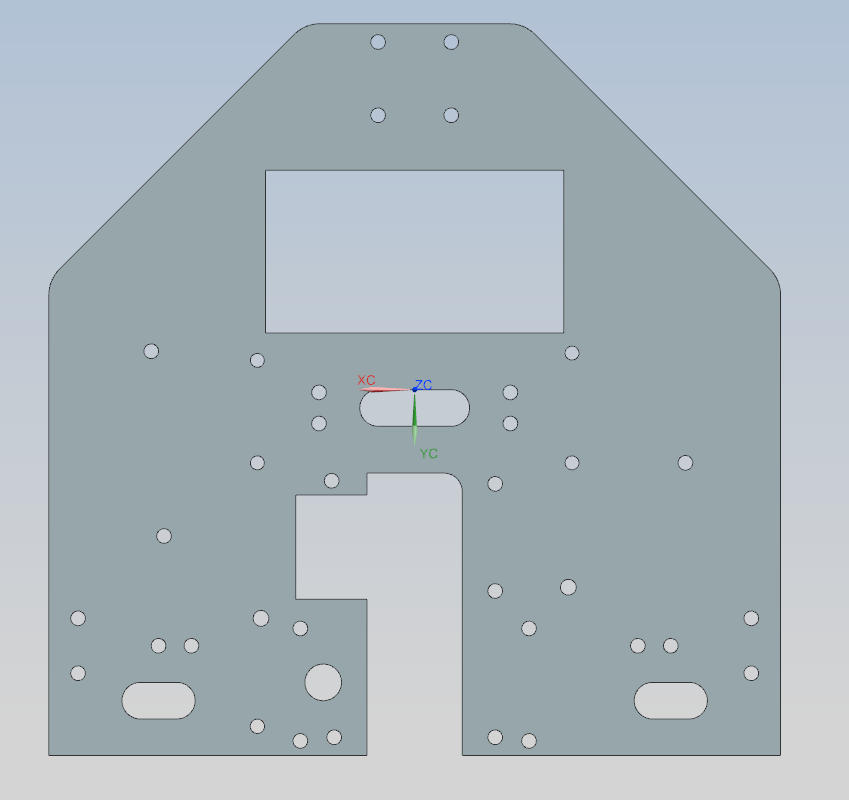
\includegraphics[width=\linewidth]{assets/MT/Grundplatte_V3.png}
        \caption{Grundplatte V3}
    \end{subfigure}
    \caption{Weiterentwicklung der Grundplatte}
    \label{fig: Weiterentwicklung der Grundplatte}
\end{figure}


\subsubsection{Recycle}

Durch die modulare Bauweise ist der Roboter nach Gebrauch auch wieder komplett zerleg
bar. Materialien und Komponenten, welche nicht wiederverwendet werden können, können einzeln recycelt werden.

\subsection{Ökobilanz und Materialanalyse}

\subsubsection{Betrachtung hinsichtlich Ökobilanz}
% Beschreibung des Gesamtgewichtes und der drei größten Material-Positionen
Das Gesamtgewicht des Fahrzeugs beträgt \textbf{1.262 Kg}. In folgender Tabelle werden die drei grössten Material-Positionen in Kilogramm und Prozent des Gesamtgewichtes aufgelistet, gefolgt von einer Beschreibung der Recyclingfähigkeit, Entsorgung und/oder Abfallbehandlung dieser Materialien.

\begin{table}[h]
\centering
\caption{Material-Positionen nach Gewichtsanteil}
\begin{tabular}{l c c p{5cm}}
\toprule
Material & Gewicht  & Anteil (\%) & Beschreibung der Recyclingfähigkeit/Entsorgung \\
\midrule
\acrshort{mdf} & 0.166 Kg & 13\% & Recycelbar aber schwierig \\
\acrshort{pla} & 0.252 Kg & 20\% & Gut Recycelbar \\
Batterie & 0.202 Kg & 16\% & Recyceln möglich aber ist teuer \\
\bottomrule
\end{tabular}
\end{table}

\subsubsection{Nachhaltig-kritischste Materialien}
% Auflistung und Beschreibung der nachhaltig-kritischsten Materialien
Im Folgenden werden mindestens drei der nachhaltig-kritischsten Materialien, die im Fahrzeug verbaut sind, aufgelistet. Für jedes Material wird erläutert, warum es nicht nachhaltig ist, und es werden mögliche Massnahmen zur Vermeidung vorgeschlagen.

\begin{itemize}
    \item \textbf{Material 1:} \acrfull{mdf} \\
          \textit{Grund der mangelnden Nachhaltigkeit:} Hoher Energieaufwand und vergleichbar hoher Leimanteil  \\
          \textit{Vermeidungsstrategie:} Leimholzplatten mit weniger Leimanteil oder Massivholzplatten verwenden. Ökolgisch zertifiziertes MDF ist nachhaltiger
          
    \item \textbf{Material 2:} Lithium in der Batterie \\
          \textit{Grund der mangelnden Nachhaltigkeit:} Lithium ist umweltschädlich bei der Herstellung. Abbau und Raffinerie benötigt viel Energie und Wasser und setzt Schadstoffe frei. \\
          \textit{Vermeidungsstrategie:} Lithium für Batterien ist praktisch nicht vermeidbar wenn eine Batterie benötigt wird. Der Herstellungsprozess kann jedoch umweltfreundlicher gestaltet werden
          
    \item \textbf{Material 3:} Kupfer in Kabel \\
          \textit{Grund der mangelnden Nachhaltigkeit:} Kupfer ist umweltschädlich bei der Herstellung. Abbau und Raffinerie benötigt viel Energie und Wasser und setzt Schadstoffe frei. \\
          \textit{Vermeidungsstrategie:} Kabel und Leitungen von Hersteller beziehen welche ausschliesslich recycletes Kupfer verwenden.
\end{itemize}

